%\documentclass[10pt]{article}
%\usepackage[utf8]{inputenc}
%\usepackage[T1]{fontenc}
%\usepackage{amsfonts}
%\usepackage{amssymb}
%\usepackage{geometry}
%\usepackage{pstricks,pst-eucl}
%\usepackage{tikz}
%\usepackage{graphics}
%\usepackage{pslatex}
%\usepackage{lscape}
%\usepackage{eurosym}
%\usepackage{skak}
%\usepackage{chessboard}

\documentclass[12pt, a4paper]{report}
%\documentclass[11pt, a4paper]{article}

%====================== PACKAGES ======================

\usepackage[french]{babel}
\frenchbsetup{StandardLists=true}
\usepackage{enumitem}
\usepackage{pifont}
\usepackage[utf8x]{inputenc}
\usepackage[T1]{fontenc}
%pour gérer les positionnement d'images
\usepackage{float}
\usepackage{amsmath}
\DeclareMathOperator{\dt}{dt}
\usepackage{graphicx}
\usepackage{tabularx}
\usepackage[colorinlistoftodos]{todonotes}
\usepackage{url}
%pour les informations sur un document compilé en PDF et les liens externes / internes
\usepackage[pdfborder=0]{hyperref}
\hypersetup{
	colorlinks = true
	}
%pour la mise en page des tableaux
\usepackage{array}
\usepackage{tabularx}
\usepackage{multirow}
\usepackage{multicol}
\setlength{\columnsep}{50pt}
%espacement entre les lignes
\usepackage{setspace}
%modifier la mise en page de l'abstract
\usepackage{abstract}
%police et mise en page (marges) du document
\usepackage[T1]{fontenc}
\usepackage[top=2cm, bottom=2cm, left=2cm, right=2cm]{geometry}
%Pour les galerie d'images
\usepackage{subfig}

\usepackage{pdfpages}
%\usepackage{tikz}

\usepackage{appendix}

\usepackage{comment}

\usepackage{skak}
\usepackage{chessboard}
%\usepackage{indentfirst}
%\usetikzlibrary{angles, quotes}
%\usetikzlibrary{decorations.pathmorphing}
%====================== INFORMATION ET REGLES ======================
%\frenchbsetup{StandardLists=false}
%rajouter les numérotation pour les \paragraphe et \subparagraphe
\setcounter{secnumdepth}{4}
\setcounter{tocdepth}{4}

\hypersetup{							% Information sur le document
pdfauthor = {Stephan Runigo},			% Auteurs
pdftitle = {Recueil d'échec},			% Titre du document
pdfsubject = {Stratégie et tactique du jeu d'échec},		% Sujet
pdfkeywords = {jeu d'échec, stratégie, tactique},	% Mots-clefs
pdfstartview={FitH}}	% ajuste la page à la largeur de l'écran
%pdfcreator = {MikTeX},% Logiciel qui a crée le document
%pdfproducer = {} % Société avec produit le logiciel
%======================== DEBUT DU DOCUMENT ========================
%
\begin{document}
%
%régler l'espacement entre les lignes
\newcommand{\HRule}{\rule{\linewidth}{0.5mm}}
%
%présentation	%
%
%
\begin{titlepage}
%
~\\[1cm]

\begin{center}
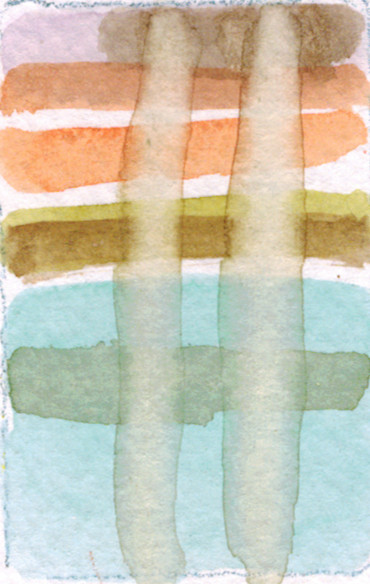
\includegraphics[scale=2]{./presentation/champ06}
\end{center}

\textsc{\Large }\\[0.5cm]

% Title \\[0.4cm]
\HRule

\begin{center}
{\huge \bfseries  Principes élémentaires\\
du jeu d'échec\\[0.4cm] }
\end{center}

\HRule \\[1.5cm]

\begin{center}
%\includegraphics[scale=0.3]{./presentation/ptoleme}
\end{center}

\begin{center}
%\includegraphics[scale=0.3]{./presentation/diagrammesInteractions}
\end{center}


% Author and supervisor
\begin{minipage}{0.4\textwidth}
\begin{flushleft} \large
\emph{Auteur:}\\
Stephan \textsc{Runigo}
\end{flushleft}
\end{minipage}
\begin{minipage}{0.4\textwidth}
\begin{flushright} \large
\emph{Illustration:}\\
Krikri
\end{flushright}
\end{minipage}

\vfill

% Bottom of the page
{\large \today}

\end{titlepage}

\newpage
\begin{center}
\Large
Résumé
\normalsize
\end{center}
\vspace{3cm}
\begin{itemize}[leftmargin=1cm, label=\ding{32}, itemsep=21pt]
\item {\bf Objet : Les ouvertures} .
\item {\bf Contenu : Principes élémentaires} .
\item {\bf Public concerné : Débutant} .
\end{itemize}

\vspace{3cm}



\vspace{3cm}


%

%
%\newpage
%~
%ne pas numéroter cette page
%\thispagestyle{empty}
	%\newpage

\tableofcontents
\thispagestyle{empty}
\setcounter{page}{0}
%ne pas numéroter le sommaire
%
%\newpage
%
%espacement entre les lignes d'un tableau
\renewcommand{\arraystretch}{1.5}
%
%====================== INCLUSION DES PARTIES ======================
%
~
\thispagestyle{empty}
%recommencer la numérotation des pages à "1"
\setcounter{page}{0}
\newpage
%
%\chapter{Problème de stratégie}
%

\newpage

\section{Énoncé des exercices}

Dans les problèmes suivant, l'analyse de la position permet de trouver un bon coup stratégique.

\subsection{Exercice 25}%%%%%%%%%%%%%%%%%%%%%%%%%%%%%%%%%%%%%%%%%%%%

\newgame
\fenboard{r4rk1/2p3b1/3p3p/p1pPp1p1/2P5/5PN1/PP4PP/1R3RK1 b − − 0 1}
\storegame{strategie25}
\begin{minipage}{0.45\textwidth}
\hspace{0.7cm}Il y a un bon coup stratégique pour les noirs.
\vspace{0.5cm}

\end{minipage}
\hfill
\begin{minipage}{0.45\textwidth}
\chessboard[
%showmover=false,
inverse,markstyle=leftborder,
]%\showboard
\end{minipage}

\subsection{Exercices 28} %%%%%%%%%%%%%%%%%%%%%%%%%%%%%%%%%%%%%%%%%%%%
\subsubsection{Exercice a} %%%%%%%%%%%%%%%%%%%%%%%%%%%%%%%%%%%%%%%%%%%%

\newgame
\fenboard{rnbqk2r/pp3ppp/2p2n2/3p2B1/1b1P4/2NB1Q2/PPP2PPP/R3K1NR b − − 0 1}
\storegame{strategie28a}
\begin{minipage}{0.45\textwidth}
\hspace{0.7cm} Ici, il y a plusieurs bon coup pour les noirs.
\vspace{0.5cm}

\hspace{0.7cm} Que joueriez-vous ?
\vspace{0.5cm}

\hspace{0.7cm} Quelle est la menace stratégique des blancs ? % Comment l'empêcher ?
\vspace{0.5cm}

\end{minipage}
\hfill
\begin{minipage}{0.45\textwidth}
\chessboard[
%showmover=false,
inverse,markstyle=leftborder,
]%\showboard
\end{minipage}

%\item 28b %%%%%%%%%%%%%%%%%%%%%%%%%%%%%%%%%%%%%%%%%%%%\subsection{28b}
\subsubsection{Exercice b} %%%%%%%%%%%%%%%%%%%%%%%%%%%%%%%%%%%%%%%%%%%%

\newgame
\fenboard{rn2k2r/pp3p2/2p1bp1p/3p4/1b1P4/P1NB1N2/1PP2PPP/R3K2R b − − 0 1}
\storegame{strategie28b}
\begin{minipage}{0.45\textwidth}
\hspace{0.7cm} Les noirs peuvent, soit échanger leur fou avec le cavalier, soit conserver leur fou.
\vspace{0.5cm}

\hspace{0.7cm} Quel est le meilleur choix ?
\vspace{0.5cm}

\end{minipage}
\hfill
\begin{minipage}{0.45\textwidth}
\chessboard[
%showmover=false,
inverse,markstyle=leftborder,
]%\showboard
\end{minipage}


%\item 28c %%%%%%%%%%%%%%%%%%%%%%%%%%%%%%%%%%%%%%%%%%%%\subsection{28c}
\subsubsection{Exercice c} %%%%%%%%%%%%%%%%%%%%%%%%%%%%%%%%%%%%%%%%%%%%

\newgame
\fenboard{r3k2r/pp1n1p2/2p1bp1p/3p4/3P4/P1PB1N2/2P2PPP/R3K2R b − − 0 1}
\storegame{strategie28c}
\begin{minipage}{0.45\textwidth}
\hspace{0.7cm}Ici, il y a un coup difficile à trouver pour les blancs. C'est un coup avec des idées, un plan.
\vspace{0.5cm}

\hspace{0.7cm} Ou se trouve la faiblesse des noirs ? Ou se trouve la faiblesse des blancs ? 
\vspace{0.5cm}

\hspace{0.7cm} Comment attaquer ces faiblesses ? Comment les défendre ? 
\vspace{0.5cm}

\end{minipage}
\hfill
\begin{minipage}{0.45\textwidth}
\chessboard
\end{minipage}

%\item 33 %%%%%%%%%%%%%%%%%%%%%%%%%%%%%%%%%%%%%%%%%%%%%%%%\subsection{33}
\subsection{Exercice 33} %%%%%%%%%%%%%%%%%%%%%%%%%%%%%%%%%%%%%%%%%%%%

\newgame
\fenboard{rn1qk2r/ppp1ppbp/3p2pn/8/2PP4/2N2P2/PP2BPPP/R1BQK2R w − − 0 1}
\storegame{strategie33}
\begin{minipage}{0.45\textwidth}
\hspace{0.7cm} Les noirs viennent de sortir leur cavalier. Quel est leur plan ?
\vspace{0.5cm}

\hspace{0.7cm} Les blancs jouent un coup qui stope le plan des noirs.
\vspace{0.5cm}

\end{minipage}
\hfill
\begin{minipage}{0.45\textwidth}
\chessboard[pgfstyle=color,
opacity=0.3,
color=green,
markfield=g8,
markfield=h6,
]
\end{minipage}
%\end{itemize}
%%%%%%%%%%%%%%%%%%%%%%%%%%%%%%%%%%%%%%%%%%%%%%%%%%%%%%%%%
%\begin{itemize}[leftmargin=0.7cm, itemsep=0pt]
%\item  \end{itemize}

%
%
%

\chapter{Finales}
%
%
%%%%%%%%%%%%%%%%%%%%%
\section{Élaboration d'un plan}
%%%%%%%%%%%%%%%%%%%%%

À la sortie de l'ouverture, nos pièces légères sont sorties, le roque à été effectué, la dame s'est dévellopée et les tours en liaison se sont placées sur les bonnes colonnes (ouvertes, semi-ouvertes, en face de la dame adverse). On entame alors le milieu de partie, et souvent, on arrive alors à la position critique. La position critique, c'est la position ou l'on ne sait plus quoi jouer. Souvent dans cette position, on fait un mauvais coup et l'adversaire en profite. Il s'agit donc de la position où l'on doit réfléchir un peu et trouver un plan.

Regarder la position de l'adversaire, détecter ses faiblesses.

Questions à se poser :

Où mes pièces seraient bien placées ? Détecter des cases faibles chez l'adversaire, quel type de pièce serait forte sur ces cases, comment ammener notre pièce sur cette cases.

Quel est ma pièce la plus mal placée ? Où serait-elle bien ?


%%%%%%%%%%%%%%%%%%%%%
\subsection{Exemples de plan}
%%%%%%%%%%%%%%%%%%%%%



\subsubsection{Exploitation d'une case faible}

On détecte une case faible dans le camp adverse et notre cavalier y serait très fort. Pour atteindre cette case,  il doit emprunter une case controlée par la dame adverse. Un de nos pion peut être poussé afin de controler cette case. Tout cela constitue un plan, 3 ou 4 coups peuvent être nécessaire à son exécution. Pendant ce temps, il faut aussi réagir aux coups de l'adversaire, contrer une menace, protéger une pièce attaquée, ... Ainsi le plan initial peut être réalisé en 8 ou 10 coups, pendant ces 8 ou 10 coups, on joue des coups en vue du plan, on sait quoi jouer. Enfin, si on y arrive, on se retrouve avec un cavalier bien placé, ce qui est un avantage.

\subsubsection{Exploitation d'un pion faible}




%%%%%%%%%%%%%%%%%%%%%%%%%%%%%%%%%%%%%%%%%%%%%%%%%%%%%%%%%%

%

\newpage

\section{Énoncé des exercices}

Dans les problèmes suivant, l'analyse de la position permet de trouver un bon coup stratégique.

\subsection{Exercice 25}%%%%%%%%%%%%%%%%%%%%%%%%%%%%%%%%%%%%%%%%%%%%

\newgame
\fenboard{r4rk1/2p3b1/3p3p/p1pPp1p1/2P5/5PN1/PP4PP/1R3RK1 b − − 0 1}
\storegame{strategie25}
\begin{minipage}{0.45\textwidth}
\hspace{0.7cm}Il y a un bon coup stratégique pour les noirs.
\vspace{0.5cm}

\end{minipage}
\hfill
\begin{minipage}{0.45\textwidth}
\chessboard[
%showmover=false,
inverse,markstyle=leftborder,
]%\showboard
\end{minipage}

\subsection{Exercices 28} %%%%%%%%%%%%%%%%%%%%%%%%%%%%%%%%%%%%%%%%%%%%
\subsubsection{Exercice a} %%%%%%%%%%%%%%%%%%%%%%%%%%%%%%%%%%%%%%%%%%%%

\newgame
\fenboard{rnbqk2r/pp3ppp/2p2n2/3p2B1/1b1P4/2NB1Q2/PPP2PPP/R3K1NR b − − 0 1}
\storegame{strategie28a}
\begin{minipage}{0.45\textwidth}
\hspace{0.7cm} Ici, il y a plusieurs bon coup pour les noirs.
\vspace{0.5cm}

\hspace{0.7cm} Que joueriez-vous ?
\vspace{0.5cm}

\hspace{0.7cm} Quelle est la menace stratégique des blancs ? % Comment l'empêcher ?
\vspace{0.5cm}

\end{minipage}
\hfill
\begin{minipage}{0.45\textwidth}
\chessboard[
%showmover=false,
inverse,markstyle=leftborder,
]%\showboard
\end{minipage}

%\item 28b %%%%%%%%%%%%%%%%%%%%%%%%%%%%%%%%%%%%%%%%%%%%\subsection{28b}
\subsubsection{Exercice b} %%%%%%%%%%%%%%%%%%%%%%%%%%%%%%%%%%%%%%%%%%%%

\newgame
\fenboard{rn2k2r/pp3p2/2p1bp1p/3p4/1b1P4/P1NB1N2/1PP2PPP/R3K2R b − − 0 1}
\storegame{strategie28b}
\begin{minipage}{0.45\textwidth}
\hspace{0.7cm} Les noirs peuvent, soit échanger leur fou avec le cavalier, soit conserver leur fou.
\vspace{0.5cm}

\hspace{0.7cm} Quel est le meilleur choix ?
\vspace{0.5cm}

\end{minipage}
\hfill
\begin{minipage}{0.45\textwidth}
\chessboard[
%showmover=false,
inverse,markstyle=leftborder,
]%\showboard
\end{minipage}


%\item 28c %%%%%%%%%%%%%%%%%%%%%%%%%%%%%%%%%%%%%%%%%%%%\subsection{28c}
\subsubsection{Exercice c} %%%%%%%%%%%%%%%%%%%%%%%%%%%%%%%%%%%%%%%%%%%%

\newgame
\fenboard{r3k2r/pp1n1p2/2p1bp1p/3p4/3P4/P1PB1N2/2P2PPP/R3K2R b − − 0 1}
\storegame{strategie28c}
\begin{minipage}{0.45\textwidth}
\hspace{0.7cm}Ici, il y a un coup difficile à trouver pour les blancs. C'est un coup avec des idées, un plan.
\vspace{0.5cm}

\hspace{0.7cm} Ou se trouve la faiblesse des noirs ? Ou se trouve la faiblesse des blancs ? 
\vspace{0.5cm}

\hspace{0.7cm} Comment attaquer ces faiblesses ? Comment les défendre ? 
\vspace{0.5cm}

\end{minipage}
\hfill
\begin{minipage}{0.45\textwidth}
\chessboard
\end{minipage}

%\item 33 %%%%%%%%%%%%%%%%%%%%%%%%%%%%%%%%%%%%%%%%%%%%%%%%\subsection{33}
\subsection{Exercice 33} %%%%%%%%%%%%%%%%%%%%%%%%%%%%%%%%%%%%%%%%%%%%

\newgame
\fenboard{rn1qk2r/ppp1ppbp/3p2pn/8/2PP4/2N2P2/PP2BPPP/R1BQK2R w − − 0 1}
\storegame{strategie33}
\begin{minipage}{0.45\textwidth}
\hspace{0.7cm} Les noirs viennent de sortir leur cavalier. Quel est leur plan ?
\vspace{0.5cm}

\hspace{0.7cm} Les blancs jouent un coup qui stope le plan des noirs.
\vspace{0.5cm}

\end{minipage}
\hfill
\begin{minipage}{0.45\textwidth}
\chessboard[pgfstyle=color,
opacity=0.3,
color=green,
markfield=g8,
markfield=h6,
]
\end{minipage}
%\end{itemize}
%%%%%%%%%%%%%%%%%%%%%%%%%%%%%%%%%%%%%%%%%%%%%%%%%%%%%%%%%
%\begin{itemize}[leftmargin=0.7cm, itemsep=0pt]
%\item  \end{itemize}

%

\newpage
%%%%%%%%%%%%%%%%%%%%%
%\chapter{Analyse}
%%%%%%%%%%%%%%%%%%%%%
\section{Analyse des exercices}

\subsection{Exercice 25}%%%%%%%%%%%%%%%%%%%%%%%%%%%%%%%%%%%%%%%%%%%%

\begin{minipage}{0.45\textwidth}
\hspace{0.7cm} Les noirs ont des pions doublées donnant deux colonnes semi-ouvertes. Les blancs ont une colonnes semi-ouvertes.

\hspace{0.7cm} Le pion a5 des noirs est faible. Le fou des noirs est un mauvais fou (les pions des noirs sont sur des cases noires) et il est inactif. Le cavalier des blanc dispose de la case e4 et rêve de la case e6

\vspace{0.15cm}
\hspace{0.7cm} Un bon coup ici est d'échanger du matériel contre de l'espace.

\vspace{0.15cm}
\hspace{0.7cm}Ou se trouve les cases faibles des noirs ? Comment y placer des pièces ?

\end{minipage}
\hfill
\begin{minipage}{0.45\textwidth}
\newgame
\restoregame{strategie25}
\chessboard[
inverse,markstyle=leftborder,
]
\end{minipage}

\subsection{Exercices 28} %%%%%%%%%%%%%%%%%%%%%%%%%%%%%%%%%%%%%%%%%%%%
\subsubsection{Exercice a} %%%%%%%%%%%%%%%%%%%%%%%%%%%%%%%%%%%%%%%%%%%%

\begin{minipage}{0.45\textwidth}
\newgame
\restoregame{strategie28a}
\chessboard[
inverse,markstyle=leftborder,
arrow=latex,
pgfstyle=straightmove,
shortenstart=0.1em,
%color=blue,
opacity=0.3,
color=green,
linewidth=3pt,
markmoves={g5-f6},
markmoves={d8-f6},
markmoves={f3-f6},
markmoves={g7-f6},
]

\hspace{0.7cm} Les blancs menacent de prendre deux fois en f6 pour détruire la structure des pions de l'aile roi.
\end{minipage}
\hfill
\begin{minipage}{0.45\textwidth}
\vspace{0.15cm}

\hspace{0.7cm} Après \mainline{1... h6 2.Bxf6 Qxf6 3.Qxf6 gxf6}

\chessboard[
inverse,markstyle=leftborder,
pgfstyle=color,
opacity=0.15,
color=red,
markfield=f7,
markfield=f6,
]

\hspace{0.35cm} Les pions doublés isolés des noirs donnent une position difficile à jouer.
\end{minipage}

\begin{minipage}{0.45\textwidth}
\end{minipage}
\hfill
\begin{minipage}{0.45\textwidth}
\end{minipage}

\subsubsection{Exercice b} %%%%%%%%%%%%%%%%%%%%%%%%%%%%%%%%%%%%%%%%%%%%

\newgame
\restoregame{strategie28b}
\begin{minipage}{0.45\textwidth}
\hspace{0.7cm} Les noirs ont une structure de pions endomagée. En contre partie ils ont la paire de fous.

\chessboard[
inverse,markstyle=leftborder,
]

\hspace{0.7cm} Si ils endommagent la structure des pions de l'aile dame des blancs par \mainline{1... Bxc3 2.bxc3}.
\vspace{0.15cm}

\end{minipage}
\hfill
\begin{minipage}{0.45\textwidth}
\chessboard[
inverse,markstyle=leftborder,
pgfstyle=color,
opacity=0.15,
color=red,
markfield=f7,
markfield=f6,
color=green,
markfield=c2,
markfield=c3,
]

\hspace{0.7cm} Les pions doublés des blancs ne sont pas faibles, ils pourront avancer et attaquer le pion central des noirs.
\vspace{0.15cm}

\hspace{0.7cm} Les pions doublés des noirs sont isolé et ne peuvent pas facilement s'échanger avec des pions blancs.
\vspace{0.15cm}

\end{minipage}

\subsubsection{Exercice c} %%%%%%%%%%%%%%%%%%%%%%%%%%%%%%%%%%%%%%%%%%%%

\begin{minipage}{0.45\textwidth}

\hspace{0.7cm} Les noirs disposent de la colonne semi-ouverte g, les blancs dispose de la colonne semi-ouverte b. La colonne e est ouverte.

\hspace{0.7cm} {\bf Des pions doublés offrent des colonnes semi-ouvertes} (de l'espace pour les tours).

\vspace{0.15cm}
\hspace{0.7cm} Les pions doublés vont être des cibles, (s'organiser pour les attaquer est un plan).

\vspace{0.15cm}
\hspace{0.7cm} Les blancs ont un bon coup stratégique pour attaquer le pion f6.

\vspace{0.15cm}
\end{minipage}
\hfill
\begin{minipage}{0.45\textwidth}
\newgame
\restoregame{strategie28c}
\chessboard[
pgfstyle=color,
color=green,
opacity=0.25,
markregion={g3-g8},
markregion={b1-b6},
color=orange,
opacity=0.25,
markregion={e1-e8},
opacity=0.25,
color=red,
markfield=f6,
]
\end{minipage}

\begin{minipage}{0.45\textwidth}
\chessboard[pgfstyle=color,
color=green,opacity=0.45,
markfield=d3,markfield=d4,
%
color=red,opacity=0.4,
markfield=e6,markfield=d5,
%
color=orange,opacity=0.3,
markfield=g4,markfield=h3,markfield=f5,
%
color=green!50!blue!50,opacity=0.4,
markfield=a6,markfield=b5,markfield=c4,
markfield=h7,markfield=g6,markfield=e4,
markfield=f1,markfield=e2,markfield=f5
%,
]
\end{minipage}
\hfill
\begin{minipage}{0.45\textwidth}

\hspace{0.7cm} Les blancs ont un bon fou (fou de case blanche et pion central sur case noire), les noirs ont un mauvais fou(fou de case blanche et pion central sur case blanche).

\vspace{0.15cm}
\hspace{0.7cm} Le fou des blancs a plus d'espace que le fou des noirs.
\vspace{0.15cm}

\vspace{0.15cm}
\end{minipage}

\begin{minipage}{0.45\textwidth}
\hspace{0.7cm} Les noirs ont des pions doublés sur la colonne f. Les blancs ont des pions doublés sur la colonne c.
% sont une faiblesse pour les noirs, 

\vspace{0.15cm}
\hspace{0.7cm} Les pions doublés des noirs sont isolés (il n'y a plus de pions noirs sur les colonnes adjacentes). ils seront difficiles à avancer.

\vspace{0.15cm}
\hspace{0.7cm} Les pions doublés des blancs seront plus facile à pousser et à échanger.

\vspace{0.15cm}
\end{minipage}
\hfill
\begin{minipage}{0.45\textwidth}
\chessboard[pgfstyle=color,
color=red,opacity=0.3,
markfield=f7,markfield=f6,
%
color=orange,opacity=0.3,
markfield=c2,markfield=c3,
]
\end{minipage}

\subsection{Exercice 33} %%%%%%%%%%%%%%%%%%%%%%%%%%%%%%%%%%%%%%%%%%%%

\newgame
\restoregame{strategie33}
\begin{minipage}{0.45\textwidth}
\hspace{0.7cm} Les noirs souhaite placer leur cavalier sur f5 pour attaquer le pion d4
\vspace{0.5cm}

\hspace{0.7cm} Si les blancs jouent le petit roque, les noir viennent attaquer le pion d4 qui est difficile à défendre sans risquer de perdre la paire de fous. 
% \mainline{1. O-O Nf5 2. Be3}
\vspace{0.5cm}

\hspace{0.7cm} Ici, les blancs ont un bon coup pour contrer le plan des noirs.
\vspace{0.5cm}

\end{minipage}
\hfill
\begin{minipage}{0.45\textwidth}
\chessboard[pgfstyle=color,
opacity=0.3,
color=green,
markfield=g8,
markfield=h6,
color=red,
markfield=f5,
]
\end{minipage}
%%%%%%%%%%%%%%%%%%%%%%%%%%%%%%%%%%%%%%%%%%%%%%%%%%%%%%%%%

%\begin{itemize}[leftmargin=1cm, label=\ding{32}, itemsep=1pt]
%\item {\bf } : \end{itemize}

%%%%%%%%%%%%%%%%%%%%%%%%%%%%%%%%%%%%%%%%%%%%%%%%%%%%%%%

%

\newpage
%%%%%%%%%%%%%%%%%%%%%
\section{Solutions}
%%%%%%%%%%%%%%%%%%%%%

\subsection{Exercice 25}%%%%%%%%%%%%%%%%%%%%%%%%%%%%%%%%%%%%%%%%%%%%
\newgame
\restoregame{strategie25}
\begin{minipage}{0.45\textwidth}
\hspace{0.7cm} Le bon coup est d'activer le fou grâce au sacrifice \mainline{1... e4}
\vspace{0.25cm}

\hspace{0.7cm} En contrepartie, le cavalier blanc arrive sur la bonne case e4 en gagnant un pion.
\vspace{0.25cm}

\hspace{0.7cm} L'activation du mauvais fou des noirs va lui permettre de rayonner sur les cases noires dans le camps des blancs. \mainline{2. Ne4 Bd4}
\vspace{0.25cm}

\hspace{0.7cm} Le plan des noir est d'attaquer sur la colonne b.
\end{minipage}
\hfill
\begin{minipage}{0.45\textwidth}
\chessboard[
%showmover=false,
inverse,markstyle=leftborder,
]
\end{minipage}

\begin{minipage}{0.45\textwidth}

{\footnotesize 
\hspace{0.7cm}Si les tours viennent à s'échanger, la finale sera favorable au noir : 
{\bf En finale fou contre cavalier, s'il y a des pions sur les deux ailes, le fou est meilleur.}

\hspace{0.7cm}{\bf Il faut rendre la position favorable pour nos pièces légères.} Si on a un fou : placer ses pions sur la couleur opposée et ouvrir la position.
}

\hspace{0.7cm} Le plan des noir est d'attaquer sur la colonne b ?
\vspace{0.25cm}

\hspace{0.7cm} \mainline{3. Kh1 Rfb8}% 4. b3 a4
\vspace{0.25cm}
\end{minipage}
\hfill
\begin{minipage}{0.45\textwidth}
\chessboard[
%showmover=false,
inverse,markstyle=leftborder,
]
\end{minipage}

\subsection{Exercices 28} %%%%%%%%%%%%%%%%%%%%%%%%%%%%%%%%%%%%%%%%%%%%
\subsubsection{Exercice a} %%%%%%%%%%%%%%%%%%%%%%%%%%%%%%%%%%%%%%%%%%%%
\newgame
\restoregame{strategie28a}
\begin{minipage}{0.45\textwidth}
\hspace{0.7cm} Le bon coup est de ramener le fou \mainline{1... Be7} afin de conserver une bonne structure de pions.

\chessboard[
inverse,markstyle=leftborder,
arrow=latex,
pgfstyle=straightmove,
shortenstart=0.1em,
%color=blue,
opacity=0.6,
color=green,
linewidth=3pt,
markmoves={b4-e7},
]

\end{minipage}
\hfill
\begin{minipage}{0.45\textwidth}
\newgame
\restoregame{strategie28a}
\hspace{0.7cm} Un autre bon coup est de développer le cavalier \mainline{1... Nbd7}.

\chessboard[
inverse,markstyle=leftborder,
arrow=latex,
pgfstyle=straightmove,
shortenstart=0.1em,
%color=blue,
opacity=0.6,
color=green,
linewidth=3pt,
markmoves={b8-d7},
]

\hspace{0.7cm} Permet de conserver la menace de détruire la structure de pions des blancs à l'aile dame mais gène la sortie du fou blanc des noirs.
\end{minipage}

\subsubsection{Exercice b} %%%%%%%%%%%%%%%%%%%%%%%%%%%%%%%%%%%%%%%%%%%%

\newgame
\restoregame{strategie28b}
\begin{minipage}{0.45\textwidth}
\hspace{0.7cm} Le bon coup est \mainline{1... Bd6}.
\vspace{0.25cm}

\hspace{0.7cm} Le cavaliers des blancs peut attaquer le pion f6 en venant sur h5. C'est un plan assez long.
\vspace{0.25cm}

\end{minipage}
\hfill
\begin{minipage}{0.45\textwidth}
\chessboard[
inverse,markstyle=leftborder,
]
\end{minipage}

\subsubsection{Exercice c} %%%%%%%%%%%%%%%%%%%%%%%%%%%%%%%%%%%%%%%%%%%%

\newgame
\restoregame{strategie28c}
\begin{minipage}{0.45\textwidth}
\hspace{0.7cm} Le bon coup est de ramener le fou \mainline{1... Be7} afin de conserver une bonne structure de pions.
\vspace{0.25cm}

\hspace{0.7cm} 23 MINUTES
\vspace{0.25cm}

\end{minipage}
\hfill
\begin{minipage}{0.45\textwidth}
\chessboard
\end{minipage}

\subsection{Exercice 33} %%%%%%%%%%%%%%%%%%%%%%%%%%%%%%%%%%%%%%%%%%%%

\newgame
\restoregame{strategie33}
\begin{minipage}{0.45\textwidth}
\hspace{0.7cm} Le bon coup est \mainline{1. g4}. Le cavalier des noirs n'a plus d'avenir (le meilleur coup pour les noirs est alors de le ramener en g8).
\vspace{0.5cm}

\hspace{0.7cm} Les blancs conserve la paire de fous. Leur bon fous (celui de case noir) possède de bonnes cases pour se développer

\end{minipage}
\hfill
\begin{minipage}{0.45\textwidth}
\chessboard
\end{minipage}

\begin{minipage}{0.45\textwidth}
\hspace{0.7cm} Si les noirs jouent le petit roque, \mainline{1... O-O}, les blancs ont une attaque après \mainline{2. h4}.
\vspace{0.5cm}

\hspace{0.7cm} Les blancs ont un avantage d'espace et le plan fou g5 et dame d2 (attaque le cavalier et donne la possibilité du grand roque).
\vspace{0.5cm}

\end{minipage}
\hfill
\begin{minipage}{0.45\textwidth}
\chessboard[arrow=latex,
pgfstyle=straightmove,
shortenstart=0.1em,
color=blue,
linewidth=3pt,
markmoves={d1-d2},
markmoves={c1-g5}
]
\end{minipage}
%%%%%%%%%%%%%%%%%%%%%%%%%%%%%%%%%%%%%%%%%%%%%%%%%%%%%%%
%\begin{itemize}[leftmargin=1cm, label=\ding{32}, itemsep=1pt]
%\item {\bf } : \end{itemize}

%
%
%

%
%%
\begin{appendix}
%

%%%%%%%%%%%%%%%%%%%%%
\chapter{Le matériel}
%%%%%%%%%%%%%%%%%%%%%


La valeur conventionnelle des pièces permet de détecter les échanges favorable.

%\multicolumn{4}{|c|}{}\\%\cline{2-7}\hline
\begin{center}
\begin{tabular}{ccc}
Pièce & valeur & cas particulier \\
Pion & 3 temps & Plus fort au centre \\
Cavalier & 3 pions & Plus fort dans les positions fermé \\
Fou & 3 pions & Plus fort dans les positions ouvertes\\
Tour & 5 pions & Forte sur les colonnes ouvertes \\
Dame & 9 pions & Plus forte en attaque qu'en défense\\
%roi &  & \\
\end{tabular}
\end{center}


%\begin{itemize}[leftmargin=1cm, label=\ding{32}, itemsep=1pt]
%\item {\bf } : \end{itemize}

%%%%%%%%%%%%%%%%%%%%%%%%%%%%%%%%%%%%%%%%%%%%%%%%%%%%%%%

%
\newpage
%

%%%%%%%%%%%%%%%%%%%%%
\chapter{L'espace}
%%%%%%%%%%%%%%%%%%%%%

%%%%%%%%%%%%%%%%%%%%%
\section{Espace contrôlé}
%%%%%%%%%%%%%%%%%%%%%

%C'est les cases accessible par les pièces (pas par les pions)

Lors de 

\begin{minipage}{0.4\textwidth}

\begin{center}
\newgame
\mainline{1. e4 }

\chessboard[color=red,
	markstyle=color,markfields=a6,
	markfields=e2,markfields=d3,markfields=c4,markfields=b5,
	markfields=f3,markfields=g4,markfields=h5,]
\end{center}
L'ouverture du pion roi offre 8 cases.
\end{minipage}
\begin{minipage}{0.5\textwidth}
\begin{center}
\newgame
\mainline{1. d4 }

\chessboard[color=red,
	markstyle=color,markfields=h6,
	markfields=d2,markfields=e3,markfields=f4,markfields=g5,
	markfields=d3,]
\end{center}
L'ouverture du pion roi offre 6 cases.
\end{minipage}

\begin{minipage}{0.4\textwidth}
\begin{center}
\newgame
\mainline{1. c4 }

\chessboard[color=red,
	markstyle=color,markfields=d4,
	markstyle=color,markfields=e5,]
\end{center}
Le cavalier f3 contrôle les deux cases centrales d4 et e5.
\end{minipage}
\begin{minipage}{0.4\textwidth}
\begin{center}
\newgame
\mainline{1. Nf3 }

\chessboard[color=red,
	markstyle=color,markfields=d4,
	markstyle=color,markfields=e5,]
\end{center}
Le cavalier f3 contrôle les deux cases centrales d4 et e5.
\end{minipage}

\newgame

\mainline{1. e4 e5 2. Nf3 Nc6}

\begin{center}
\chessboard
\end{center}

%\newchessgame
\newgame

\def\empharea{ h8-f4 }
\chessboard[emphstyle=\color{red},
empharea=\empharea]


%%%%%%%%%%%%%%%%%%%%%
%\section{Le temps}
%%%%%%%%%%%%%%%%%%%%%

\fenboard{r5k1/1b1p1ppp/p7/1p1Q4/2p1r3/PP4Pq/BBP2b1P/R4R1K w − − 0 20}
\mbox{}
\bigskip
\showboard
\mainline{20.Qxb7 Rae8 21.Qd5}





%\newgame
%\mainline{1. Nf3 }
%\def\empharea{ f3-f3 }
%\chessboard[color=red,
%	markstyle=color,markfields=d4,
%	markstyle=color,markfields=e5,
%	emphstyle=\color{green},
%	empharea=\empharea]
%%%%%%%%%%%%%%%%%%%%%%%%%%%%%%%%%%%%%%%%%%%%%%%%%%%%%%%

%
\newpage
%

%%%%%%%%%%%%%%%%%%%%%
\chapter{Le temps}
%%%%%%%%%%%%%%%%%%%%%

%%%%%%%%%%%%%%%%%%%%%
%\section{L'espace}
%%%%%%%%%%%%%%%%%%%%%

C'est les cases accessible par les pièces (pas par les pions)

e4 offre 8 cases, e5 offre 6 cases.


C'est le nombres de mouvement de pièces pour atteindre la position.

%\begin{itemize}[leftmargin=1cm, label=\ding{32}, itemsep=1pt]
%\item {\bf } : \end{itemize}




\fenboard{r5k1/1b1p1ppp/p7/1p1Q4/2p1r3/PP4Pq/BBP2b1P/R4R1K w − − 0 20}

\mbox{}
\bigskip

\showboard


\mainline{20.Qxb7 Rae8 21.Qd5}







%%%%%%%%%%%%%%%%%%%%%%%%%%%%%%%%%%%%%%%%%%%%%%%%%%%%%%%

%
\newpage
%
%\input{./annexe/.tex}
%
\newpage
%
\end{appendix}
%

%
%====================== INCLUSION DE LA BIBLIOGRAPHIE ======================
%
%récupérer les citation avec "/footnotemark"
%\nocite{*}
%choix du style de la biblio
\bibliographystyle{plain}
%inclusion de la biblio
\cleardoublepage
\addcontentsline{toc}{chapter}{Bibliographie}
\bibliography{bibliographie.bib}
%\newpage
%\input{./glossaire/glossaire.tex}
%\newpage
%\input{./annexes/annexes.tex}
\end{document}
%%%%%%%%%%%%%%%%%%%%%%%%%%%%%%%%%%%%%%%%%%%%%%%%%%%%%%%%%%%%%%%%%%%%%%%%%%%%%%%%%
